\chapter{近似算法}

\begin{introduction}
	\item 近似算法介绍
	\item 顶点覆盖
	\item 任务调度
	\item 最小带权覆盖
	\item MAX-K-SAT
\end{introduction}

本章讲述了NPC问题的一些近似算法及其质量分析。

\section{近似算法介绍}

\subsection{引入与定义}

求解NPC问题的思路通常包括:
\begin{enumerate}
	\item 设计通用的指数级时间复杂度算法
	\item 针对特例设计多项式时间复杂度算法
	\item 根据问题特点设计启发式算法,或借用元启发式算法的框架求解(如蚁群、遗传、退火等算法)
	\item 设计近似算法
\end{enumerate}
其中设计近似算法时便要求时间复杂度是多项式级,得到的解可以保证与最优解比差别有限,具体定义如下。

\begin{definition}{近似算法}{approximation-algorithm:15Ln-ApproximationAlgorithm}
	对一个问题有多项式级时间复杂度,并对任意实例均有$ALG\leqslant \alpha \cdot OPT$,其中$\alpha$为一个常数,则称该算法为此问题的近似算法。(ALG为该算法结果的质量,OPT为最优解的质量)
\end{definition}

\subsection{近似算法常用证明方法}

\begin{figure}[htb]
	\centering
	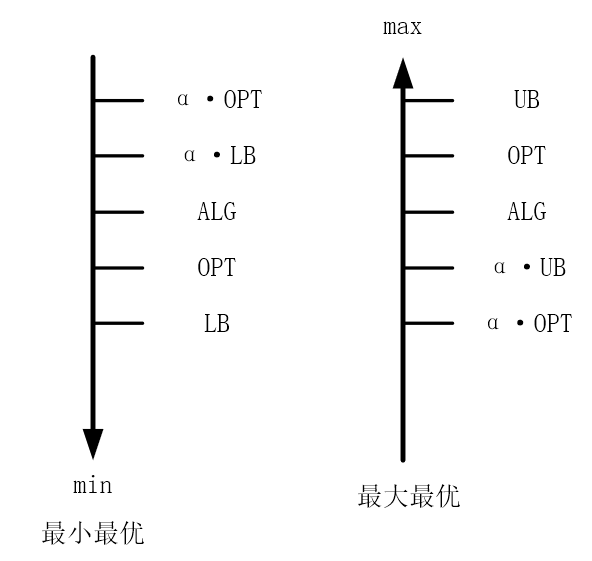
\includegraphics[scale=0.3]{image/Ln15-ApproximationAlgorithm1.png}
	\caption{近似算法证明思路}\label{proof:Ln15-ApproximationAlgorithm}
\end{figure}

\subsubsection{最小最优证明}
一般利用\autoref{proof:Ln15-ApproximationAlgorithm}的证明思路,首先找到OPT下界LB,证明$OPT\geqslant LB$,再想办法证明$ALG\leqslant \alpha \cdot LB$,从而得到$ALG\leqslant \alpha \cdot OPT$,即可证明该近似算法的正确性。
\subsubsection{最大最优证明}
同样利用\autoref{proof:Ln15-ApproximationAlgorithm}的证明思路,首先找到OPT上界UB,证明$OPT\leqslant UB$,再想办法证明$ALG\geqslant \alpha \cdot UB$,从而得到$ALG\geqslant \alpha \cdot OPT$,即可证明该近似算法的正确性。



\section{顶点覆盖}

本节将介绍一个顶点覆盖的近似算法。

\subsection{问题描述}

\begin{definition}{顶点覆盖问题}{vertex-cover:15Ln-ApproximationAlgorithm}
	对于给定的图$(V,E)$,找到一个点集$S\subset V$,使得该图所有边都至少有一个端点在点集S中。
\end{definition}

\subsection{算法描述}

算法步骤如下:
\begin{enumerate}
	\item 找到极大匹配M,相关定义如下:
	\begin{definition}{匹配}{matching:15Ln-ApproximationAlgorithm}
		给定一个图G,在G的一个子图M中,任意两边都没有相同的端点,且每个点都有边相连。
	\end{definition}
	\begin{definition}{极大匹配}{maximal-matching:15Ln-ApproximationAlgorithm}
		一个匹配无法再增加任何点和边,则称之为极大匹配。
	\end{definition}
	\item 输出M中的所有点作为解的点集S
\end{enumerate}

\subsection{正确性证明}

\begin{proposition}{求证}{proof1:15Ln}
该算法始终有$ALG\leqslant 2\cdot OPT$,在该问题中OTP即为最优解点的数量,ALG即为算法求解的点的数量。
\end{proposition}
证明:
\begin{enumerate}
	\item 证明$OPT\geqslant |M|$(其中|M|为极大匹配的边数):对于M中任意一条边,其必定至少有一点在OPT中,否则这条边就未被覆盖,与顶点覆盖的要求矛盾。故$OPT\geqslant |M|$
	\item 证明$ALG=2\cdot |M|$:极大匹配中任意一点度为1,故点的数量即为边的数量的两倍,得证$ALG=2\cdot |M|$。
	\item 根据上述证明可以得到$2\cdot OPT\geqslant 2\cdot|M|=ALG$,得证$ALG\leqslant 2\cdot OPT$
\end{enumerate}
	
\section{任务调度}

\section{最小带权覆盖}

本节将介绍一个最小带权覆盖的近似算法。

\subsection{问题描述}

\begin{definition}{最小带权覆盖问题}{weighted-vertex-cover:15Ln-ApproximationAlgorithm}
	对于给定的图$(V,E)$,各个点有权重w,找到一个点集$S\subset V$,使得该图所有边都至少有一个端点在点集S中,且S中所有点的权重之和比所有可行的解都小。
\end{definition}

\subsection{算法描述}

算法步骤如下:
\begin{enumerate}
	\item 将原问题建模为线性规划问题:原问题是$\forall e=(u,v)\epsilon E$,有$v\epsilon S$或$u\epsilon S$,求$\min \sum_{v\epsilon G} x_vw_v$其中
	\[
		x_v = \begin{cases}
			0 & v\notin S \\
			1 & v\epsilon S
		\end{cases}
	\]\\
	将其转化为线性规划问题,可变为:
	\[
		\begin{cases}
			x_v^*+x_u^*\geqslant 1 			   &\forall e=(u,v)\epsilon E\\
			x_v^*\geqslant 0	   			   &\forall v\epsilon G, x_v\epsilon [0,1]\\
			\min \sum_{v\epsilon G} x_v^*w_v &\forall v\epsilon G\
		\end{cases}
	\]
	\item 使用线性规划求解器求解,再将得到的解转化为原问题的解:
	\[
		x_v=\begin{cases}
			0 &x_v^*<0.5\\
			1 &x_v^*\geqslant 0.5
		\end{cases}
	\]
\end{enumerate}

\subsection{正确性证明}

\begin{proposition}{求证}{proof2:15Ln}
	该算法得到的解是一个顶点覆盖
\end{proposition}
证明:
	因为$\forall e=(u,v)\epsilon E,x_v^*+x_u^*\geqslant 1$,故$x_v^*\geqslant 0.5$或$x_u^*\geqslant 0.5$,故$x_v$和$x_u$至少有一个为1,即至少有一点覆盖该边e。
\begin{proposition}{求证}{proof3:15Ln}
	$ALG\leqslant 2\cdot OPT$
\end{proposition}
证明:
	$OPT\geqslant \sum_{v\epsilon G} x_v^*w_v^*$,而又有$x_v\leqslant 2\cdot x_v^*$,故有
	$ALG=\sum_{v\epsilon G} x_vw_v\leqslant 2\cdot \sum_{v\epsilon G} x_v^*w_v^*\leqslant 2\cdot OPT$,得证。

\section{MAX-K-SAT}


本节将介绍一个最小带权覆盖的近似算法。

\subsection{问题描述}

\begin{definition}{最小带权覆盖问题}{weighted-vertex-cover:15Ln-ApproximationAlgorithm}
	对于给定的图$(V,E)$,各个点有权重w,找到一个点集$S\subset V$,使得该图所有边都至少有一个端点在点集S中,且S中所有点的权重之和比所有可行的解都小。
\end{definition}

\subsection{算法描述}

算法步骤如下:
\begin{enumerate}
	
\end{enumerate}

\subsection{正确性证明}

\begin{proposition}{求证}{proof2:15Ln}
	该算法得到的解是一个顶点覆盖
\end{proposition}
证明:
	因为$\forall e=(u,v)\epsilon E,x_v^*+x_u^*\geqslant 1$,故$x_v^*\geqslant 0.5$或$x_u^*\geqslant 0.5$,故$x_v$和$x_u$至少有一个为1,即至少有一点覆盖该边e。
\begin{proposition}{求证}{proof3:15Ln}
	$ALG\leqslant 2\cdot OPT$
\end{proposition}
证明:
	$OPT\geqslant \sum_{v\epsilon G} x_v^*w_v^*$,而又有$x_v\leqslant 2\cdot x_v^*$,故有
	$ALG=\sum_{v\epsilon G} x_vw_v\leqslant 2\cdot \sum_{v\epsilon G} x_v^*w_v^*\leqslant 2\cdot OPT$,得证。

这是一段代码:

\begin{lstlisting}[language=Python, caption=Python example]
import numpy as np

def incmatrix(genl1,genl2):
    m = len(genl1)
    n = len(genl2)
    M = None #to become the incidence matrix
    VT = np.zeros((n*m,1), int)  #dummy variable

    #compute the bitwise xor matrix
    M1 = bitxormatrix(genl1)
    M2 = np.triu(bitxormatrix(genl2),1)

    for i in range(m-1):
        for j in range(i+1, m):
            [r,c] = np.where(M2 == M1[i,j])
            for k in range(len(r)):
                VT[(i)*n + r[k]] = 1;
                VT[(i)*n + c[k]] = 1;
                VT[(j)*n + r[k]] = 1;
                VT[(j)*n + c[k]] = 1;

                if M is None:
                    M = np.copy(VT)
                else:
                    M = np.concatenate((M, VT), 1)

                VT = np.zeros((n*m,1), int)

    return M
\end{lstlisting}

更多环境请见文档。

\section{引用}

\subsection{交叉引用}

引用定理~\ref{thm:label-for-this-theorem}。

\subsection{参考文献}

引用一个参考文献~\cite{cormen2009introduction}
